\documentclass[11pt,a4paper,titlepage]{article}

% --- Paquets essentiels ---
\usepackage[utf8]{inputenc}
\usepackage[T1]{fontenc}
\usepackage[french]{babel}
\usepackage{lmodern}
\usepackage{microtype}
\usepackage{geometry}
\geometry{a4paper, top=2.5cm, bottom=2.5cm, left=2.5cm, right=2.5cm, headheight=14pt}

\usepackage{graphicx}
\usepackage{float}
\graphicspath{{images/}{docs/images/}{../docs/images/}}
\usepackage{xcolor}
\usepackage{booktabs}
\usepackage{tabularx}
\usepackage{array}
\usepackage{multirow}
\usepackage{amsmath,amssymb}
\usepackage{fancyhdr}
\usepackage{titlesec}
\usepackage{caption}
\captionsetup{skip=5pt, belowskip=8pt}
% Adjust spacing for figures and text
\setlength{\textfloatsep}{10pt}
\setlength{\floatsep}{12pt}
\setlength{\intextsep}{10pt}
\setlength{\parskip}{6pt}
\renewcommand{\baselinestretch}{1.2}
\captionsetup{skip=5pt, belowskip=8pt}
\usepackage{subcaption}
\usepackage{tcolorbox}
\tcbuselibrary{skins,breakable}
\usepackage{listings}
\usepackage{enumitem}
\usepackage{hyperref}

% --- Palette de couleurs professionnelles ---
\definecolor{emsiGreen}{RGB}{0, 102, 68}
\definecolor{emsiDarkGreen}{RGB}{0, 70, 46}
\definecolor{emsiAccent}{RGB}{230, 81, 0}
\definecolor{primaryBlue}{RGB}{24, 76, 120}
\definecolor{darkText}{RGB}{33, 37, 41}
\definecolor{lightGray}{RGB}{248, 249, 250}
\definecolor{borderGray}{RGB}{222, 226, 230}
\definecolor{boxBg}{RGB}{245, 248, 250}
\definecolor{boxBorder}{RGB}{180, 205, 225}

% --- Configuration Hyperref ---
\hypersetup{
    colorlinks=true,
    linkcolor=emsiDarkGreen,
    citecolor=emsiAccent,
    filecolor=primaryBlue,
    urlcolor=emsiDarkGreen,
    pdfauthor={Hamza Arhrid, Issam Bouffa},
    pdftitle={EMSICollab - Cadre Général, Méthodologie Agile & Conception UML},
    pdfsubject={Rapport Académique d'Ingénierie Logicielle},
    pdfkeywords={EMSI, Microservices, UML, Scrum, PlantUML, Matching, PFE}
}

% --- Configuration des En-têtes et Pieds de page ---
\pagestyle{fancy}
\fancyhf{}
\fancyhead[L]{\small\color{gray}\textsc{EMSICollab} -- Architecture \& Conception}
\fancyhead[R]{\small\color{gray}\nouppercase{\leftmark}}
\fancyfoot[L]{\small\color{gray}Hamza ARHRID \& Issam BOUFFA -- EMSI 2026/2027}
\fancyfoot[R]{\small\color{gray}Page \thepage}
\renewcommand{\headrulewidth}{0.4pt}
\renewcommand{\footrulewidth}{0.4pt}

% --- Titres de sections personnalisés ---
\titleformat{\section}
  {\normalfont\Large\bfseries\color{emsiDarkGreen}}{\thesection}{1em}{}[{\titlerule[1pt]}]
\titleformat{\subsection}
  {\normalfont\large\bfseries\color{primaryBlue}}{\thesubsection}{1em}{}
\titleformat{\subsubsection}
  {\normalfont\normalsize\bfseries\color{darkText}}{\thesubsubsection}{1em}{}

% --- Boîtes d'alertes & remarques ---
\newtcolorbox{calloutbox}[2][]{
    enhanced,
    breakable,
    colback=boxBg,
    colframe=emsiDarkGreen,
    arc=3mm,
    boxrule=1pt,
    left=4mm, right=4mm, top=3mm, bottom=3mm,
    title=\textbf{#2},
    coltitle=white,
    colbacktitle=emsiDarkGreen,
    #1
}

\newtcolorbox{featurebox}[1]{
    enhanced,
    breakable,
    colback=lightGray,
    colframe=primaryBlue,
    arc=2mm,
    boxrule=0.8pt,
    title=\textbf{#1},
    coltitle=white,
    colbacktitle=primaryBlue,
    left=3mm, right=3mm, top=2mm, bottom=2mm
}

% --- Configuration des Listings de Code ---
\lstset{
    basicstyle=\ttfamily\small,
    backgroundcolor=\color{lightGray},
    keywordstyle=\color{primaryBlue}\bfseries,
    stringstyle=\color{emsiAccent},
    commentstyle=\color{gray}\itshape,
    frame=single,
    rulecolor=\color{borderGray},
    breaklines=true,
    showstringspaces=false,
    tabsize=2,
    captionpos=b
}

% =========================================================================
% DOCUMENT PRINCIPAL
% =========================================================================
\begin{document}

% -------------------------------------------------------------------------
% PAGE DE GARDE OFFICIELLE
% -------------------------------------------------------------------------
\begin{titlepage}
    \begin{center}
        \vspace*{-0.5cm}
        
\includegraphics[height=2.2cm]{images/emsi_logo.jpg}\\[0.3cm]
        {\Large \textbf{ÉCOLE MAROCAINE DES SCIENCES DE L'INGÉNIEUR}}\\[0.2cm]
        {\large Filière Ingénierie Informatique et Réseaux (IIR)}\\[1.5cm]
        
        \rule{\linewidth}{1.5pt}\\[0.5cm]
        {\Huge \bfseries \color{emsiDarkGreen} EMSICollab}\\[0.3cm]
        {\Large \bfseries \color{primaryBlue} Plateforme Microservices Intelligente de Gestion de Projets Académiques, Matching de Compétences \& Espaces Collaboratifs}\\[0.3cm]
        \rule{\linewidth}{1.5pt}\\[1.5cm]
        
        {\large \textbf{Rapport de Cadre Général, Méthodologie Agile \& Modélisation UML Détaillée}}\\[1.8cm]

        \begin{minipage}{0.52\textwidth}
            \begin{flushleft} \large
                \textbf{Réalisé par :}\\
                \textbf{Hamza ARHRID} \& \textbf{Issam BOUFFA}\\
                Élèves-Ingénieurs en Informatique
            \end{flushleft}
        \end{minipage}
        \hfill
        \begin{minipage}{0.48\textwidth}
            \begin{flushright} \large
                \textbf{Sous la direction de :}\\
                Corps Professoral EMSI\\
                Département d'Ingénierie Logicielle
            \end{flushright}
        \end{minipage}

        \vfill
        {\large Année Universitaire : 2026 -- 2027}\\[0.3cm]
        {\small Version 2.0 -- Spécifications \& Conception Intégrale}
    \end{center}
\end{titlepage}

% -------------------------------------------------------------------------
% TABLE DES MATIÈRES & LISTES
% -------------------------------------------------------------------------
\tableofcontents
\newpage
\listoffigures
\listoftables
\newpage

% =========================================================================
% PARTIE I : CADRE GÉNÉRAL & MÉTHODOLOGIE
% =========================================================================
\section{Cadre Général \& Méthodologie}

\subsection{Analyse de l'Existant}

La réalisation des Projets de Fin d'Études (PFE) et des projets d'ingénierie au sein des grandes écoles supérieures comme l'EMSI représente un jalon crucial de la formation. Toutefois, le processus traditionnel de formation d'équipes et de suivi académique souffre de limitations organisationnelles notables :
\begin{itemize}[leftmargin=1.5cm]
    \item Constitution manuelle ou par affinité informelle, conduisant à des déséquilibres critiques de profils (ex. 4 profils backend sans compétences UI/UX ou DevOps).
    \item Manque de visibilité globale sur les compétences techniques réelles des étudiants.
    \item Éparpillement des supports de communication (WhatsApp, Slack, emails informels) rendant le suivi pédagogique opaque et difficile à évaluer pour l'enseignant.
    \item Suivi discontinu de l'avancement avec des réunions improvisées et sans journalisation formelle des jalons.
\end{itemize}

\subsubsection{Étude Comparative (Benchmarking des Solutions Actuelles)}

Afin de situer notre apport technologique, nous avons conduit une étude comparative rigoureuse des plateformes de gestion de projets et d'équipes les plus répandues sur le marché :

Afin d'évaluer la pertinence de développer une plateforme dédiée, nous avons conduit un benchmarking rigoureux sur six solutions représentatives du marché : Trello, Jira Software, GitHub Projects, Google Classroom, Zoom Video Communications et notre solution EMSICollab :

\begin{table}[htbp]
\centering
\scriptsize
\caption{Étude Comparative Exhaustive : Trello, Jira, GitHub, Google Classroom, Zoom vs EMSICollab}
\label{tab:benchmarking}
\begin{tabularx}{\textwidth}{p{3.2cm} c c c c c >{\bfseries\color{emsiDarkGreen}}c}
\toprule
\textbf{Critère / Fonctionnalité} & \textbf{Trello} & \textbf{Jira} & \textbf{GitHub} & \textbf{Classroom} & \textbf{Zoom} & \textbf{EMSICollab} \\
\midrule
\textbf{Gestion PFE / Projets académiques} & \textcolor{red}{\texttimes} & \textcolor{red}{\texttimes} & \textcolor{red}{\texttimes} & \textcolor{orange}{Partiel} & \textcolor{red}{\texttimes} & \textcolor{emsiGreen}{\checkmark Natif} \\
\addlinespace
\textbf{Profilage \& Radar de compétences} & \textcolor{red}{\texttimes} & \textcolor{red}{\texttimes} & \textcolor{orange}{Partiel} & \textcolor{red}{\texttimes} & \textcolor{red}{\texttimes} & \textcolor{emsiGreen}{\checkmark Radar 1 à 5} \\
\addlinespace
\textbf{Algorithme de matching \& Veto} & \textcolor{red}{\texttimes} & \textcolor{red}{\texttimes} & \textcolor{red}{\texttimes} & \textcolor{red}{\texttimes} & \textcolor{red}{\texttimes} & \textcolor{emsiGreen}{\checkmark Pondéré + Veto} \\
\addlinespace
\textbf{Flux de recommandation PFE} & \textcolor{red}{\texttimes} & \textcolor{red}{\texttimes} & \textcolor{red}{\texttimes} & \textcolor{red}{\texttimes} & \textcolor{red}{\texttimes} & \textcolor{emsiGreen}{\checkmark Feed personnalisé} \\
\addlinespace
\textbf{Cahier des charges PDF intégré} & \textcolor{orange}{Pièce jointe} & \textcolor{orange}{Ticket} & \textcolor{orange}{Fichier Git} & \textcolor{orange}{Lien Drive} & \textcolor{red}{\texttimes} & \textcolor{emsiGreen}{\checkmark Visionneuse PDF} \\
\addlinespace
\textbf{Roadmap interactif (\% dynamique)} & \textcolor{orange}{Checklist} & \textcolor{orange}{Sprints} & \textcolor{orange}{Milestones} & \textcolor{orange}{Devoirs} & \textcolor{red}{\texttimes} & \textcolor{emsiGreen}{\checkmark Checkboxes + \%} \\
\addlinespace
\textbf{Chatroom dédiée (Icône carte projet)} & \textcolor{red}{\texttimes} & \textcolor{red}{\texttimes} & \textcolor{red}{\texttimes} & \textcolor{orange}{Flux général} & \textcolor{orange}{Team Chat} & \textcolor{emsiGreen}{\checkmark WebSocket 1 clic} \\
\addlinespace
\textbf{Messagerie privée 1-à-1} & \textcolor{red}{\texttimes} & \textcolor{red}{\texttimes} & \textcolor{red}{\texttimes} & \textcolor{orange}{Gmail} & \textcolor{orange}{Chat direct} & \textcolor{emsiGreen}{\checkmark Chat direct} \\
\addlinespace
\textbf{Planification Réunions \& Visio} & \textcolor{red}{Plugin tiers} & \textcolor{red}{Plugin tiers} & \textcolor{red}{\texttimes} & \textcolor{orange}{Meet classe} & \textcolor{emsiGreen}{\checkmark Visio seule} & \textcolor{emsiGreen}{\checkmark Meet ciblé projet} \\
\addlinespace
\textbf{Architecture technique} & SaaS & SaaS/DC & SaaS Cloud & Workspace & SaaS Cloud & \textcolor{emsiGreen}{\checkmark Microservices} \\
\bottomrule
\end{tabularx}
\end{table}

\subsubsection{Synthèse des Limites des Outils Existants}
\begin{enumerate}[leftmargin=1cm]
    \item \textbf{Inadéquation au contexte académique :} Les outils d'entreprise (Jira) imposent une complexité de paramétrage disproportionnée pour un semestre universitaire, sans lien avec le plan d'études ou la validation d'enseignants.
    \item \textbf{Absence de synergie algorithmique :} Aucun outil n'analyse la complémentarité des compétences entre membres pour garantir qu'une équipe dispose de l'ensemble des prérequis exigés par le sujet.
    \item \textbf{Dispersion des outils de suivi :} La séparation entre les tâches, les documents de cadrage (PDF), la discussion textuelle et les séances de visio engendre des pertes d'information continues.
\end{enumerate}

\subsubsection{Valeurs Ajoutées d'EMSICollab}
EMSICollab introduit une rupture méthodologique et technique à travers six piliers :
\begin{itemize}[leftmargin=1.5cm]
    \item \textbf{Moteur de Matching Algorithmique (\texttt{SkillMatchingEngine}) :} Calcul d'un score d'adéquation pondéré ($Score \in [0, 100\%]$) et application stricte de \textbf{règles de veto} sur les compétences obligatoires.
    \item \textbf{Dashboard Étudiant \& Constitution Dynamique d'Équipe :} Ajout d'équipiers en direct avec simulation instantanée de l'éligibilité face aux sujets PFE.
    \item \textbf{Cadrage Structuré avec Cahier des Charges PDF :} Chaque sujet comporte une description pédagogique détaillée et son document officiel PDF téléchargeable ou consultable en ligne.
    \item \textbf{Suivi d'Avancement par Jalons à Cases à Cocher :} Découpage du projet en étapes séquentielles. Chaque case cochée met à jour dynamiquement la jauge globale d'avancement ($Avancement\% = \frac{\text{validées}}{\text{total}} \times 100$).
    \item \textbf{Espaces Collaboratifs Intégrés :} Une \textbf{Chatroom de projet} accessible en un clic directement depuis l'icône de la carte projet, combinée à une \textbf{messagerie privée instantanée 1-à-1}.
    \item \textbf{Planification de Réunions à Date Fixe \& Google Meet :} L'enseignant programme des revues d'avancement précises avec bouton de téléportation directe dans la salle de visio Google Meet.
\end{itemize}

\newpage
\subsection{Méthodologie de Gestion de Projet}

\subsubsection{Approche Agile (Scrum)}
Le développement de la plateforme EMSICollab s'appuie sur la méthodologie Agile **Scrum**, articulée autour d'itérations courtes de deux semaines (Sprints), permettant de livrer des incréments logiciels fonctionnels, testés et déployables.

\paragraph{Rôles Scrum Définis :}
\begin{itemize}[leftmargin=1.5cm]
    \item \textbf{Product Owner (PO) :} Définit la vision produit, priorise le Product Backlog, rédige les critères d'acceptation (User Stories) et valide les livrables à chaque fin d'itération.
    \item \textbf{Scrum Master (SM) :} Garant de l'application des rituels agiles, veille à éliminer les obstacles techniques et organisationnels, et maintient la vélocité de l'équipe.
    \item \textbf{Équipe de Développement (DEV Team) :} Ingénieurs pluridisciplinaires responsables de la conception technique, du développement fullstack (Spring Boot microservices / React SPA) et des tests unitaires/E2E.
\end{itemize}

\paragraph{Artefacts Scrum :}
\begin{itemize}[leftmargin=1.5cm]
    \item \textbf{Product Backlog :} Liste hiérarchisée des fonctionnalités attendues, continuellement affinée.
    \item \textbf{Sprint Backlog :} Sélection des User Stories engagées pour le sprint courant avec leur décomposition en tâches techniques.
    \item \textbf{Incrément Produit :} Version stable de l'application déployée sur l'environnement de staging, respectant la \textit{Definition of Done} (DoD).
\end{itemize}

\paragraph{Cérémonies Scrum Rythmées :}
\begin{itemize}[leftmargin=1.5cm]
    \item \textbf{Sprint Planning :} Planification collective au lancement du sprint (estimation en Story Points via Planning Poker).
    \item \textbf{Daily Scrum :} Point quotidien de 15 minutes synchronisant l'avancement et dégageant les blocages.
    \item \textbf{Sprint Review :} Démonstration de l'incrément logiciel fonctionnel aux parties prenantes (corps professoral EMSI).
    \item \textbf{Sprint Retrospective :} Analyse rétrospective visant l'amélioration continue des processus et de l'architecture.
\end{itemize}

\subsubsection{Signification de « A1 - 2 Agilité »}
Dans le cadre de l'ingénierie EMSI, l'annotation **« A1 - 2 Agilité »** caractérise :
\begin{enumerate}[leftmargin=1cm]
    \item \textbf{Axe 1 -- Niveau d'Agilité Opérationnelle (Niveau 2 / Mature) :} L'équipe applique un Scrum structuré avec automatisation CI/CD, tests automatisés systématiques et mesure rigoureuse de la vélocité.
    \item \textbf{Axe 2 -- Agilité \& Automatisation Intelligente :} Intégration de l'agilité au sein même de la plateforme EMSICollab, où les étapes d'avancement (Roadmap Checkboxes) et le calcul dynamique des scores de matching s'adaptent instantanément aux évolutions du projet.
\end{enumerate}

\subsubsection{Scrum vs Kanban \& Justification du Choix de Scrumban}
\begin{table}[htbp]
\centering
\small
\caption{Comparatif Analytique : Scrum, Kanban et Choix Hybride Scrumban}
\label{tab:scrum-kanban}
\begin{tabularx}{\textwidth}{l p{4.2cm} p{4.2cm} >{\bfseries\color{emsiDarkGreen}}p{4.2cm}}
\toprule
\textbf{Caractéristique} & \textbf{Scrum Pur} & \textbf{Kanban Pur} & \textbf{Approche Retenue : Scrumban} \\
\midrule
\textbf{Cadence} & Sprints fixes (2 semaines) & Flux continu sans itérations & Sprints de 2 semaines avec flux tiré \\
\addlinespace
\textbf{Gestion des tâches} & Engagées par Sprint Backlog & Limites d'en-cours (WIP Limits) & Backlog cadencé + WIP Limits \\
\addlinespace
\textbf{Adaptabilité} & Changements au sprint suivant & Changements en temps réel & Adaptabilité rapide aux retours enseignants \\
\addlinespace
\textbf{Métriques} & Vélocité, Burndown Chart & Lead Time, Cycle Time & Vélocité + Cycle Time des microservices \\
\addlinespace
\textbf{Pertinence EMSI} & Idéal pour les jalons académiques & Idéal pour la maintenance d'API & \textcolor{emsiGreen}{Idéal : respect des soutenances et flexibilité microservices} \\
\bottomrule
\end{tabularx}
\end{table}

\noindent\textbf{Justification du Choix :} Le modèle hybride **Scrumban** offre le meilleur équilibre : il préserve le cadre temporel strict imposé par le calendrier académique de l'EMSI (dates butoirs de soutenance et jalons de validation) tout en conférant la fluidité nécessaire au développement asynchrone des microservices.

\newpage
\subsection{Planning Prévisionnel \& Diagramme de Gantt}

\subsubsection{Découpage des Sprints et Jalons Académiques}
Le calendrier de développement s'étale sur 16 semaines découpées en 6 phases clés :
\begin{itemize}[leftmargin=1.5cm]
    \item \textbf{Sprint 0 (15 Sep -- 06 Oct) : Cadrage \& Infrastructure}
    \begin{itemize}
        \item Étude comparative, benchmarking et expression des besoins.
        \item Conception de l'architecture microservices et schéma des bases de données.
        \item Mise en place du monorepo, Docker Compose et socle de conteneurs.
        \item \textbf{Jalon 1 (06 Oct) : Validation de l'Architecture Technique.}
    \end{itemize}
    \item \textbf{Sprint 1 (05 Oct -- 26 Oct) : Sécurité \& Profils de Compétences}
    \begin{itemize}
        \item Développement de \texttt{auth-service} (Spring Boot 3, JWT 0.12.6, BCrypt).
        \item Gestion du catalogue des compétences techniques et seed des données.
        \item Frontend React : mire de connexion EMSI et composant Radar Chart.
        \item \textbf{Jalon 2 (26 Oct) : MVP Authentification \& Profilage.}
    \end{itemize}
    \item \textbf{Sprint 2 (26 Oct -- 16 Nov) : Gestion des Sujets, PDF \& Jalons}
    \begin{itemize}
        \item Développement de \texttt{project-service} (CRUD sujets, exigences pondérées).
        \item Module de téléversement et consultation du Cahier des Charges PDF.
        \item Roadmap de projet à étapes séquentielles avec cases à cocher interactives.
        \item \textbf{Jalon 3 (16 Nov) : Sujets \& Roadmap Opérationnels.}
    \end{itemize}
    \item \textbf{Sprint 3 (16 Nov -- 07 Déc) : Moteur de Matching Algorithmique}
    \begin{itemize}
        \item Développement de \texttt{team-matching-service}.
        \item Implémentation de \texttt{SkillMatchingEngine} avec règles de veto strictes.
        \item Dashboard étudiant : constitution d'équipe et feed de recommandations PFE.
        \item \textbf{Jalon 4 (07 Déc) : Moteur de Matching Validé.}
    \end{itemize}
    \item \textbf{Sprint 4 (07 Déc -- 28 Déc) : Espaces Collaboratifs \& Google Meet}
    \begin{itemize}
        \item Développement de \texttt{chat-service} (WebSocket STOMP sur SockJS).
        \item Intégration de la Chatroom de projet (icône sur la carte) et messagerie privée.
        \item Module de planification de réunions et intégration des liens Google Meet.
        \item \textbf{Jalon 5 (28 Déc) : Espace Collaboratif Complet.}
    \end{itemize}
    \item \textbf{Sprint 5 (28 Déc -- 12 Jan) : Recette, Tests \& Soutenance Finale}
    \begin{itemize}
        \item Tests de charge, tests d'intégration E2E et monitoring via Actuator.
        \item Rédaction finale du rapport technique et livrables d'ingénierie.
        \item \textbf{Livrable Ultime (12 Jan) : Soutenance Finale devant le Jury d'Examen.}
    \end{itemize}
\end{itemize}

\subsubsection{Diagramme de Gantt du Projet}

La figure \ref{fig:gantt_planning} illustre l'ordonnancement temporel, les interdépendances et les jalons critiques de l'ensemble du projet :

\begin{figure}[htbp]
    \centering
    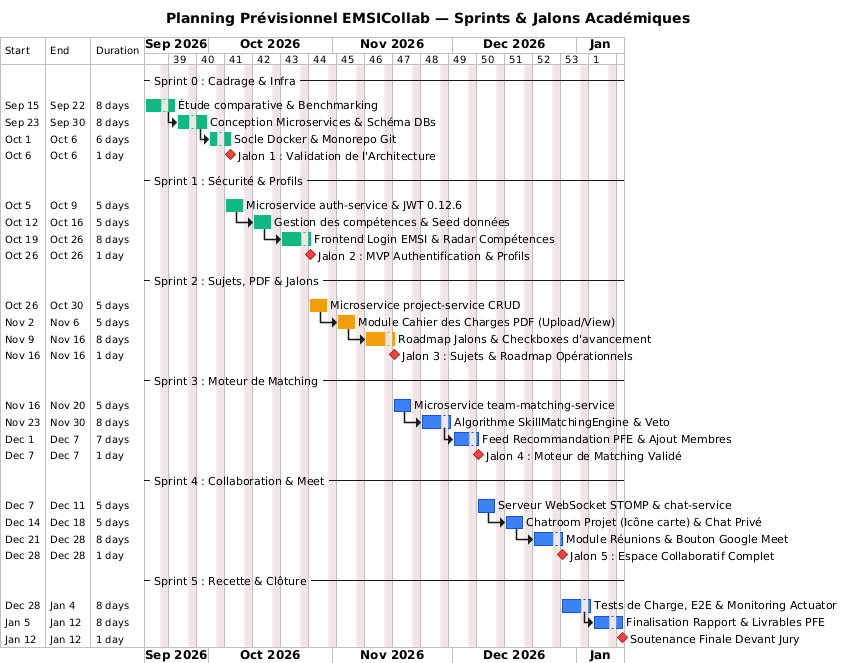
\includegraphics[width=\textwidth]{images/gantt_planning.png}
    \caption{Planning Prévisionnel Gantt -- Sprints, Tâches et Jalons Académiques EMSICollab}
    \label{fig:gantt_planning}
\end{figure}

\newpage
% =========================================================================
% PARTIE II : ANALYSE ET CONCEPTION DU PROJET (MODÉLISATION UML)
% =========================================================================
\section{Analyse et Conception du Projet (Modélisation UML)}

\subsection{Diagrammes des Cas d'Utilisation (Use Case — 3 Parties)}

\subsubsection{Identification des Acteurs Système}

Le système EMSICollab interagit avec quatre acteurs clairement différenciés :
\begin{itemize}[leftmargin=1.5cm]
    \item \textbf{Étudiant (\texttt{STUDENT}) :} Acteur principal. Il s'authentifie, déclare ses compétences, explore les sujets, forme une équipe, simule son matching, coche les jalons de la roadmap et rejoint les réunions Google Meet.
    \item \textbf{Professeur Encadrant (\texttt{PROFESSOR}) :} Publie les sujets PFE, joint le PDF du cahier des charges, définit les exigences pondérées et les vetos, valide les équipes et planifie les réunions de suivi.
    \item \textbf{Administrateur (\texttt{ADMIN}) :} Gère les comptes, importe les promotions CSV, maintient le référentiel des compétences et surveille l'état des microservices.
    \item \textbf{Moteur Algorithmique (\texttt{Système}) :} Évalue les scores d'adéquation, applique les règles de veto bloquantes et recalcule la progression globale (\%).
\end{itemize}

% ---- UC PARTIE 1 ----
\newpage
\subsubsection{Partie 1 — Sécurité, Authentification \& Profils de Compétences}

\begin{calloutbox}{Packages couverts}
\textbf{Package 1 :} Authentification JWT, gestion du profil utilisateur, déclaration des compétences (niveau 1–5) et visualisation du Radar Chart d'expertise individuelle.\\[4pt]
\textbf{Acteurs :} Étudiant · Professeur Encadrant · Administrateur
\end{calloutbox}

\vspace{10pt}
\begin{figure}[H]
    \centering
    \fbox{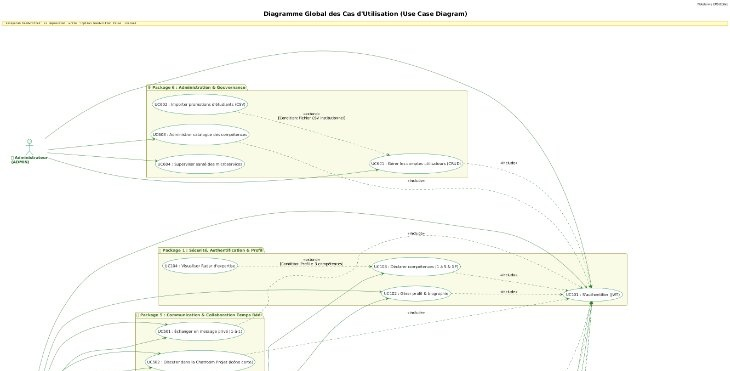
\includegraphics[width=0.88\textwidth]{images/use_case_part1.jpg}}
    \caption{Use Case — Partie 1 : Sécurité, Authentification \& Profils de Compétences}
    \label{fig:uc_part1}
\end{figure}

% ---- UC PARTIE 2 ----
\newpage
\subsubsection{Partie 2 — Sujets PFE, Cahier des Charges PDF \& Matching d'Équipe}

\begin{calloutbox}{Packages couverts}
\textbf{Package 2 :} Publication des sujets PFE, attachement du PDF officiel, définition des exigences pondérées ($w_i$) et règles de veto.\\[4pt]
\textbf{Package 3 :} Création d'équipe, ajout de membres, simulation algorithmique de compatibilité avec déclenchement du veto bloquant si compétence obligatoire manquante.\\[4pt]
\textbf{Acteurs :} Étudiant · Professeur Encadrant · Moteur Algorithmique
\end{calloutbox}

\vspace{10pt}
\begin{figure}[H]
    \centering
    \fbox{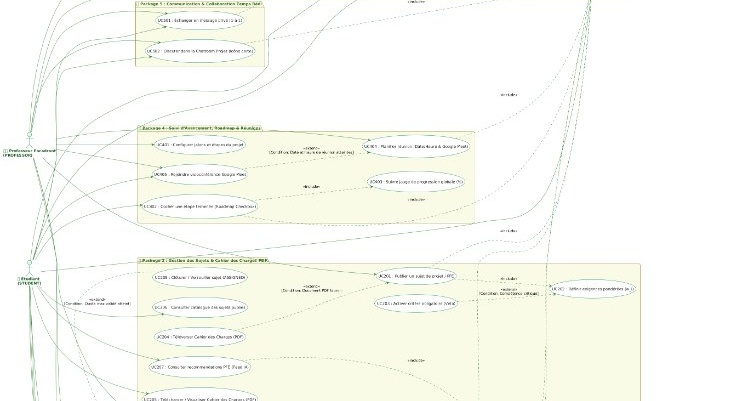
\includegraphics[width=0.88\textwidth]{images/use_case_part2.jpg}}
    \caption{Use Case — Partie 2 : Sujets PFE, Cahier des Charges PDF \& Matching d'Équipe}
    \label{fig:uc_part2}
\end{figure}

% ---- UC PARTIE 3 ----
\newpage
\subsubsection{Partie 3 — Suivi d'Avancement, Google Meet \& Collaboration Temps Réel}

\begin{calloutbox}{Packages couverts}
\textbf{Package 4 :} Configuration des jalons de roadmap, validation par checkbox, recalcul instantané de la jauge de progression (\%) et planification des réunions à date fixe avec lien Google Meet.\\[4pt]
\textbf{Package 5 \& 6 :} Chatroom de projet (icône sur la carte), messagerie privée 1-à-1, administration des comptes, import CSV et monitoring des microservices.\\[4pt]
\textbf{Acteurs :} Étudiant · Professeur Encadrant · Administrateur
\end{calloutbox}

\vspace{10pt}
\begin{figure}[H]
    \centering
    \fbox{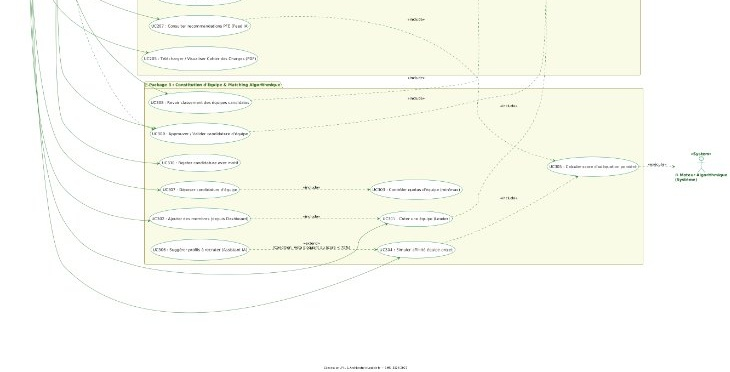
\includegraphics[width=0.88\textwidth]{images/use_case_part3.jpg}}
    \caption{Use Case — Partie 3 : Suivi d'Avancement, Google Meet \& Collaboration}
    \label{fig:uc_part3}
\end{figure}

\newpage
\subsection{Diagrammes de Séquence Système (Sequence Diagrams)}

Nous avons modélisé avec précision les 6 scénarios critiques de la plateforme afin d'illustrer la chronologie des flux entre le client React SPA, la passerelle API Gateway, les microservices Spring Boot et la couche de persistance PostgreSQL.

\subsubsection{Scénario 1 : Authentification JWT, Profilage \& Radar de Compétences}
Ce scénario décrit la connexion d'un étudiant avec vérification du domaine académique, l'émission du token JWT signé HMAC-SHA256 et le chargement des compétences pour générer le diagramme Radar interactif.

\begin{figure}[htbp]
    \centering
    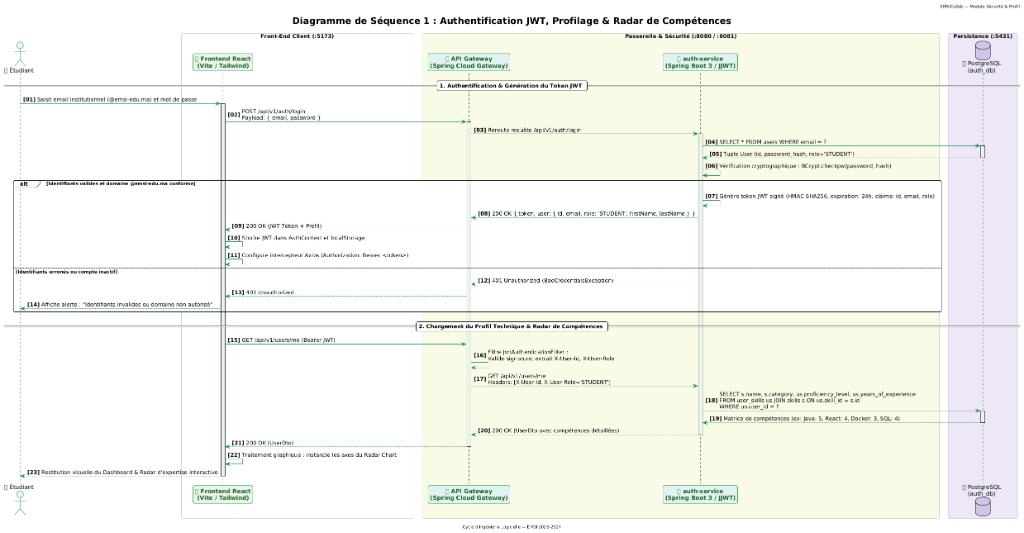
\includegraphics[width=0.98\textwidth]{images/sequence_01_auth_radar.jpg}
    \caption{Diagramme de Séquence 1 : Authentification JWT, Profilage \& Radar de Compétences}
    \label{fig:seq_auth}
\end{figure}

\newpage
\subsubsection{Scénario 2 : Publication de Sujet avec Exigences Pondérées \& Cahier des Charges PDF}
Ce scénario illustre la publication d'un sujet PFE par un enseignant. Il détaille le téléversement multipart du fichier PDF officiel du cahier des charges, la persistance des exigences avec leurs pondérations et l'émission d'un événement asynchrone sur le bus Kafka.

\begin{figure}[htbp]
    \centering
    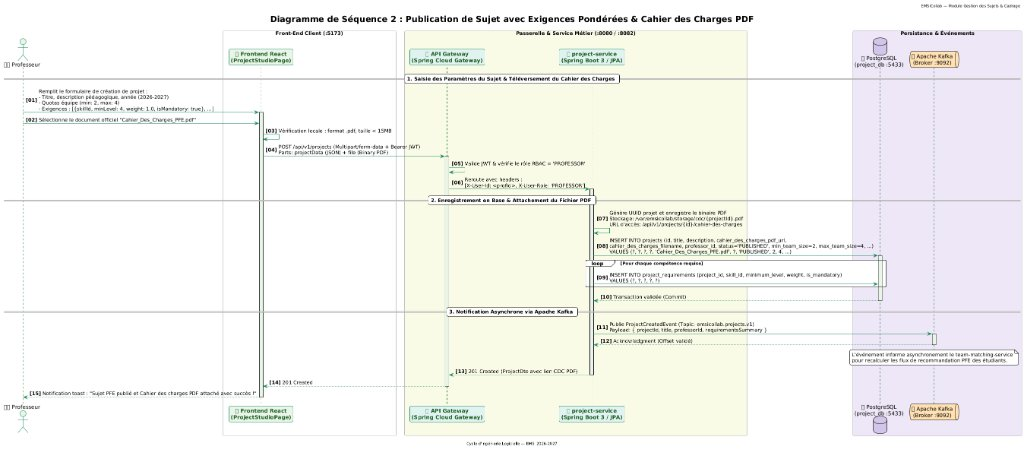
\includegraphics[width=0.98\textwidth]{images/sequence_02_publish_project_pdf.jpg}
    \caption{Diagramme de Séquence 2 : Publication de Sujet \& Attachement du Cahier des Charges PDF}
    \label{fig:seq_pdf}
\end{figure}

\newpage
\subsubsection{Scénario 3 : Constitution d'Équipe \& Simulation de Matching avec Règle de Veto}
Ce scénario met en évidence le fonctionnement de l'algorithme de matching : le chef d'équipe ajoute un camarade depuis son dashboard, lance la simulation face à un sujet, et le moteur évalue les compétences avec déclenchement immédiat de l'alerte Veto en cas de compétence critique manquante.

\begin{figure}[htbp]
    \centering
    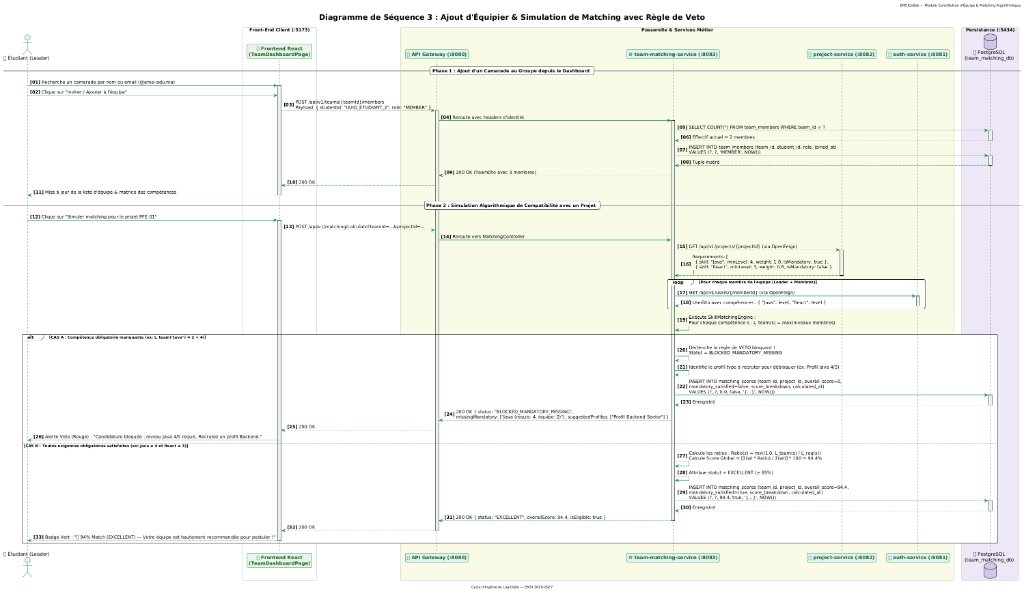
\includegraphics[width=0.98\textwidth]{images/sequence_03_team_matching_veto.jpg}
    \caption{Diagramme de Séquence 3 : Constitution d'Équipe \& Simulation de Matching avec Règle de Veto}
    \label{fig:seq_veto}
\end{figure}

\newpage
\subsubsection{Scénario 4 : Collaboration en Chatroom de Projet (Icône Carte Projet)}
Ce scénario détaille le protocole d'échange temps réel : clic sur l'icône chatroom sur la carte projet, négociation du handshake WebSocket avec passage en protocole STOMP, chargement de l'historique et diffusion instantanée des messages aux étudiants et à l'encadrant.

\begin{figure}[htbp]
    \centering
    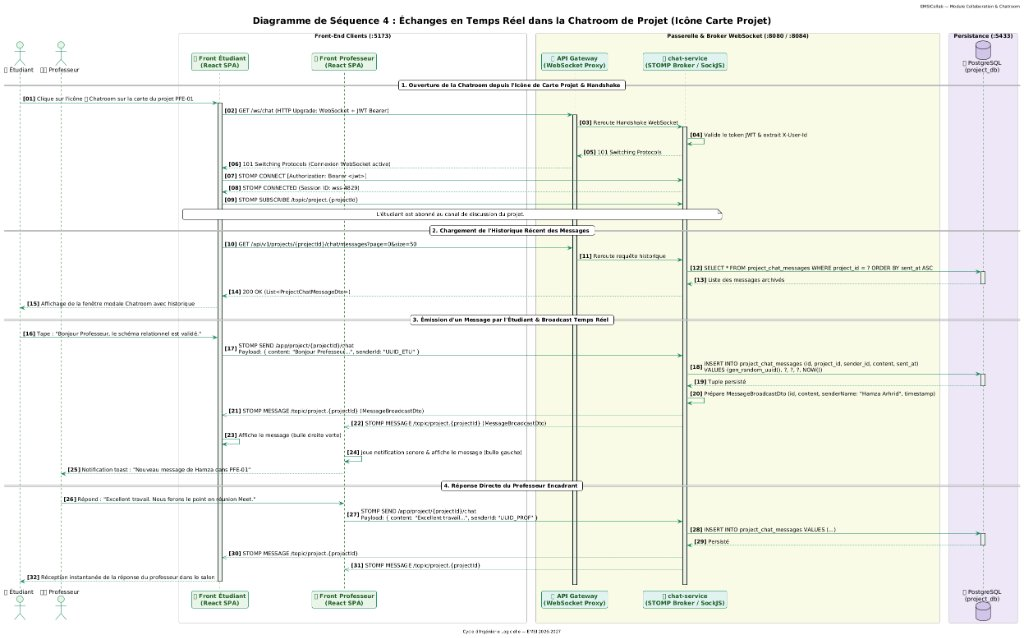
\includegraphics[width=0.98\textwidth]{images/sequence_04_project_chatroom.jpg}
    \caption{Diagramme de Séquence 4 : Échanges Temps Réel dans la Chatroom de Projet}
    \label{fig:seq_chatroom}
\end{figure}

\newpage
\subsubsection{Scénario 5 : Validation d'Étape par Checkbox \& Recalcul de Progression}
Ce scénario montre le dynamisme du suivi d'avancement : un étudiant coche une case d'étape dans la roadmap, le backend persiste l'identité de l'auteur et l'horodatage, recalcule immédiatement le pourcentage global du projet et diffuse l'état actualisé en temps réel via WebSocket.

\begin{figure}[htbp]
    \centering
    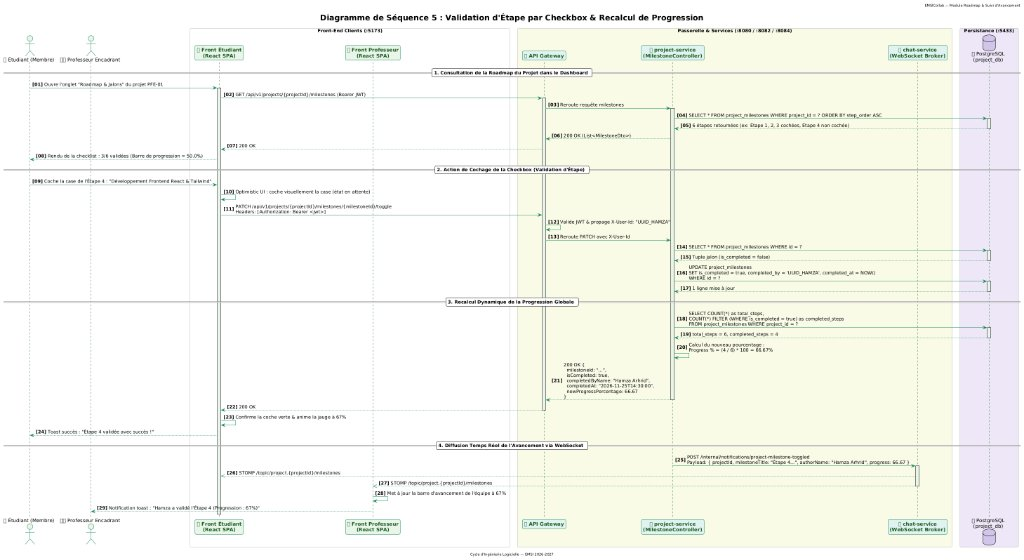
\includegraphics[width=0.98\textwidth]{images/sequence_05_milestones_checkboxes.jpg}
    \caption{Diagramme de Séquence 5 : Validation d'Étape par Checkbox \& Recalcul de Progression}
    \label{fig:seq_checkboxes}
\end{figure}

\newpage
\subsubsection{Scénario 6 : Planification de Réunion à Date Fixe \& Connexion Google Meet}
Ce scénario illustre l'organisation des séances pédagogiques : l'enseignant renseigne la date, l'heure et le lien Google Meet, l'étudiant voit apparaître un bandeau dynamique sur son dashboard 15 minutes avant l'échéance et accède en 1 clic à la visioconférence.

\begin{figure}[htbp]
    \centering
    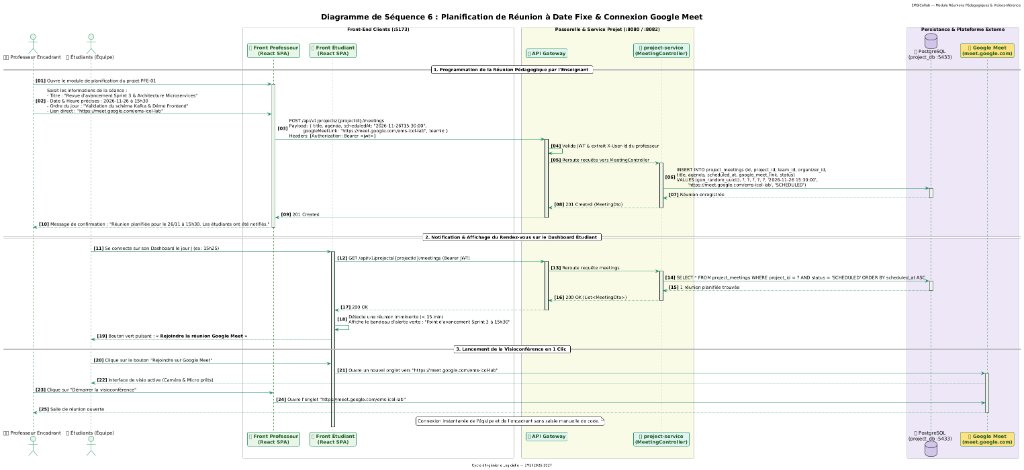
\includegraphics[width=0.98\textwidth]{images/sequence_06_meetings_google_meet.jpg}
    \caption{Diagramme de Séquence 6 : Planification de Réunion à Date Fixe \& Connexion Google Meet}
    \label{fig:seq_meet}
\end{figure}

\newpage
\subsection{Diagramme de Classes du Domaine (3 Parties — Bounded Contexts)}

Dans l'esprit du patron d'architecture \textbf{Database-per-Service}, chaque microservice possède son propre modèle de données isolé. Le diagramme de classes est présenté en \textbf{3 parties modulaires} correspondant aux 3 Bounded Contexts principaux.

% ---- CLASS PARTIE 1 ----
\newpage
\subsubsection{Partie 1 — Sécurité, Utilisateurs \& Compétences (\texttt{auth-service :8081})}

\begin{calloutbox}{Classes du Bounded Context auth-service}
\textbf{Entités :} \texttt{User} · \texttt{Role} · \texttt{Skill} · \texttt{SkillCategory} · \texttt{UserSkill}\\[4pt]
\textbf{Rôle :} Administre l'identité cryptographique (JWT/RBAC), la matrice de compétences individuelles ($niveau \in [1,5]$, années d'expérience) et le Radar Chart interactif.
\end{calloutbox}

\vspace{10pt}
\begin{figure}[H]
    \centering
    \fbox{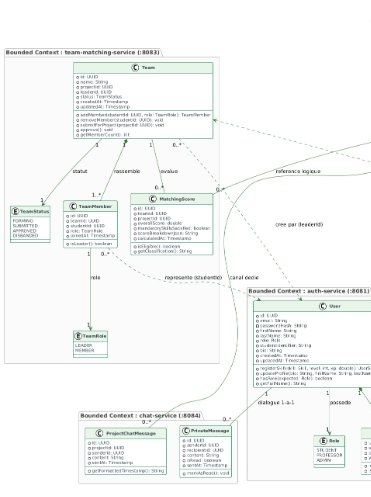
\includegraphics[width=0.88\textwidth]{images/class_part1.jpg}}
    \caption{Classes — Partie 1 : Sécurité, Utilisateurs \& Compétences (\texttt{auth-service})}
    \label{fig:class_part1}
\end{figure}

% ---- CLASS PARTIE 2 ----
\newpage
\subsubsection{Partie 2 — Sujets, Cahier des Charges, Jalons \& Meet (\texttt{project-service :8082})}

\begin{calloutbox}{Classes du Bounded Context project-service}
\textbf{Entités :} \texttt{Project} · \texttt{ProjectStatus} · \texttt{ProjectRequirement} · \texttt{ProjectMilestone} · \texttt{ProjectMeeting} · \texttt{MeetingStatus}\\[4pt]
\textbf{Rôle :} Supervise le cycle de vie des projets, le PDF officiel du cahier des charges, les exigences pondérées ($w_i$), la roadmap à cocher (\texttt{isCompleted}) et les séances Google Meet.
\end{calloutbox}

\vspace{10pt}
\begin{figure}[H]
    \centering
    \fbox{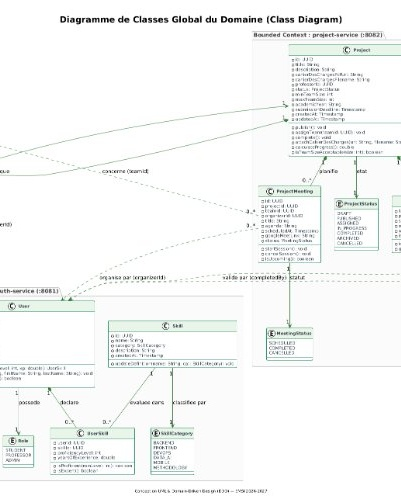
\includegraphics[width=0.88\textwidth]{images/class_part2.jpg}}
    \caption{Classes — Partie 2 : Sujets, Jalons \& Réunions Google Meet (\texttt{project-service})}
    \label{fig:class_part2}
\end{figure}

% ---- CLASS PARTIE 3 ----
\newpage
\subsubsection{Partie 3 — Équipes, Matching Algorithmique \& Chat (\texttt{team-matching} \& \texttt{chat-service})}

\begin{calloutbox}{Classes des Bounded Contexts team-matching-service \& chat-service}
\textbf{Entités (matching) :} \texttt{Team} · \texttt{TeamStatus} · \texttt{TeamMember} · \texttt{TeamRole} · \texttt{MatchingScore}\\[4pt]
\textbf{Entités (chat) :} \texttt{ProjectChatMessage} · \texttt{PrivateMessage}\\[4pt]
\textbf{Rôle :} Calcule le score d'adéquation pondéré, applique la clause d'exclusion veto (\texttt{isMandatory=true}) et assure la persistance des messages WebSocket STOMP.
\end{calloutbox}

\vspace{10pt}
\begin{figure}[H]
    \centering
    \fbox{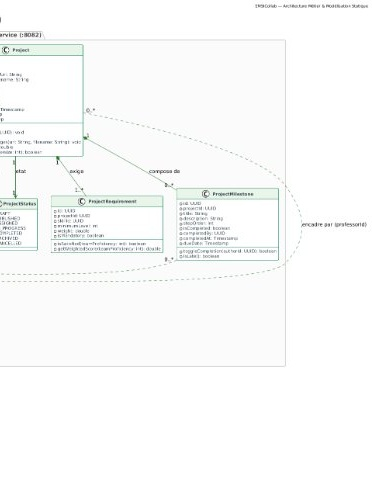
\includegraphics[width=0.88\textwidth]{images/class_part3.jpg}}
    \caption{Classes — Partie 3 : Matching d'Équipe \& Collaboration (\texttt{team-matching} \& \texttt{chat-service})}
    \label{fig:class_part3}
\end{figure}

\newpage
\subsubsection{Dictionnaire des Classes et Responsabilités}

\begin{table}[htbp]
\centering
\small
\caption{Dictionnaire des Classes du Domaine Métier}
\label{tab:classes_dict}
\begin{tabularx}{\textwidth}{l l p{8.5cm}}
\toprule
\textbf{Entité Métier} & \textbf{Microservice} & \textbf{Responsabilité Principale} \\
\midrule
\texttt{User} & \texttt{auth-service} & Représente tout acteur du système (Étudiant, Professeur, Admin) avec ses identifiants et sa biographie. \\
\addlinespace
\texttt{Skill} & \texttt{auth-service} & Compétence technique normalisée (Spring, React, Docker) rattachée à une catégorie d'ingénierie. \\
\addlinespace
\texttt{UserSkill} & \texttt{auth-service} & Association qualifiant le niveau d'expertise ($1$ à $5$) et l'expérience de l'étudiant. \\
\addlinespace
\texttt{Project} & \texttt{project-service} & Sujet PFE publié par l'enseignant avec contraintes d'effectif et \textbf{cahier des charges PDF}. \\
\addlinespace
\texttt{ProjectRequirement} & \texttt{project-service} & Exigence technique caractérisée par un niveau minimal, un poids $w_i$ et un indicateur veto. \\
\addlinespace
\texttt{ProjectMilestone} & \texttt{project-service} & Étape de roadmap avec case à cocher (\textbf{checkbox}), horodatage et auteur de validation. \\
\addlinespace
\texttt{ProjectMeeting} & \texttt{project-service} & Rendez-vous de suivi pédagogique planifié avec date fixe et \textbf{lien Google Meet direct}. \\
\addlinespace
\texttt{Team} & \texttt{team-matching} & Équipe d'étudiants constituée depuis le dashboard pour candidater à un projet. \\
\addlinespace
\texttt{TeamMember} & \texttt{team-matching} & Appartenance d'un élève-ingénieur à une équipe avec rôle (\texttt{LEADER} ou \texttt{MEMBER}). \\
\addlinespace
\texttt{MatchingScore} & \texttt{team-matching} & Résultat de l'évaluation algorithmique : score global en \%, conformité aux règles de veto. \\
\addlinespace
\texttt{ProjectChatMessage} & \texttt{chat-service} & Message diffusé en WebSocket STOMP dans la chatroom dédiée de la carte projet. \\
\addlinespace
\texttt{PrivateMessage} & \texttt{chat-service} & Message textuel instantané confidentiel échangé en 1-à-1 entre deux utilisateurs. \\
\bottomrule
\end{tabularx}
\end{table}

\newpage
% =========================================================================
% CONCLUSION
% =========================================================================
\section{Conclusion \& Perspectives}

Ce document de conception a établi les fondements méthodologiques et architecturaux de la plateforme **EMSICollab**. 

Grâce à l'application de la démarche **Scrumban**, le projet bénéficie à la fois d'une planification prévisionnelle rigoureuse respectant les jalons académiques de l'EMSI et de la flexibilité nécessaire au développement d'un écosystème microservices distribué.

La modélisation UML intégrale -- décomposée en cas d'utilisation par packages, diagrammes de séquence chronologiques couvrant l'ensemble des interactions temps réel (WebSocket, Kafka) et diagrammes de classes cloisonnés par Bounded Context -- garantit une implémentation robuste, modulaire et hautement évolutive. Les innovations clés telles que le \textbf{moteur de matching avec veto}, l'intégration du \textbf{cahier des charges PDF officiel}, le suivi dynamique par \textbf{checkboxes d'avancement}, la \textbf{chatroom de projet} et les \textbf{réunions Google Meet} répondent directement aux problématiques réelles de gestion des projets d'ingénierie au sein de l'École Marocaine des Sciences de l'Ingénieur.

\end{document}